\documentclass[../main.tex]{subfiles}

\graphicspath{{../images/}}

\begin{document}
\pagestyle{fancy}
\lhead{Lecture 3: 9/3/24}
\chead{Chapter 2}
\rhead{PHYS 421}

\section{Electrostatics}
\barh \vspace{1em}

\subsection{The Electric Field}

given charge $q$: find force on $Q$ , where $\vb F$ depends on $\boldscriptr, \vb v_i, \vb a_i$

\subsubsection{Coulombs law}

Coulomb's Law empirically,
\[\vb F_Q = \ke \frac{qQ}{\scriptr^2} \vu\scriptr\]
where $k = \frac{1}{4\pi\epsilon_0}$ and the permittivity of free space is $\epsilon_0 = \qty{8.85e-12}{C^2/Nm^2}$

\paragraph*{} The force is attractive if $sgn(qQ) = -1$ and repulsive if $= +1$.

\paragraph*{Principal of superposition:}
\begin{align*}
    \vb F_T &= \vb F_{Q1} + \vb F_{Q2} + \dots \\
    &= \ke Q \qt(\frac{q_1}{\scriptr_1^2} \vu\scriptr_1 + \frac{q_2}{\scriptr_2^2} \vu\scriptr_2 + \dots) \\
    &= Q \vb E_T
\end{align*}
where $\vb E_T$ is the total electric field due to all of the source (point) charges.

\paragraph*{}$\vb E$ doesn't depend on $Q$
\begin{itemize}
    \item $\vb E \sim F/Q$
\end{itemize}

\paragraph*{Example:} $\vb E$ field midway above two charges $q$:
\begin{figure*}[ht]
    \centering
    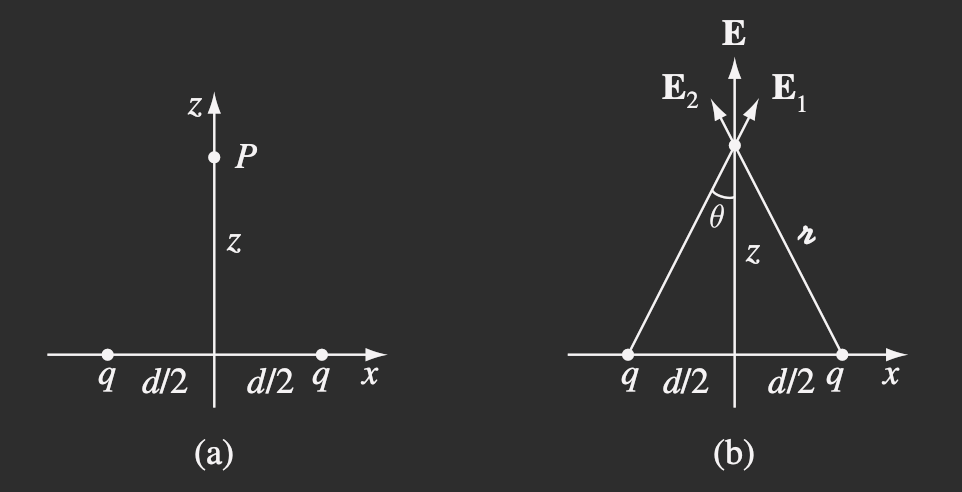
\includegraphics[width=0.5\textwidth]{ex2_1.png}
    \caption{Griffiths Example 2.1}
\end{figure*}
The electric fields are zero in the $x$ and $y$ direction:
\[E_x = E_y = 0\]
But we can sum the fields in the $z$ direction:
\[E_z = 2 \ke \frac{q}{\scriptr^2}{\cos\theta}\]
where
\[\scriptr = \qt[z^2 + \qt(\frac{d}{2})^2]^{1/2} \quad \cos\theta = \frac{z}{\scriptr}\]
so
\begin{align*}
    E_z &= \ke \frac{2qz}{\qt[z^2 + \qt(\frac{d}{2})^2]^{3/2}}
\end{align*}
Far away: $z \gg d$, so $d \to 0$ thus
\begin{align*}
    E_z &\approx \ke \frac{2qz}{z^3} = \ke \frac{2}{z^2}
\end{align*}

\paragraph*{Continuous Charge Distributions}

\begin{itemize}
    \item line: charge per unit length $\lambda; \quad \dd q = \lambda \dd \ell$
    \item surface: charge per unit area $\sigma; \quad \dd q = \sigma \dd a$
    \item volume: charge per unit volume $\rho; \quad \dd q = \rho \dd \tau$
\end{itemize}
\[\vb E(\vb r) = \ke \int \frac{1}{\scriptr^2} \vu\scriptr \dd q\]
e.g. for a volume charge:
\[\vb E(\vb r) = \ke \int \frac{\rho(\vb r')}{\scriptr^2} \vu\scriptr \dd \tau'\]
where $'$ denotes the source charge in (no $'$ is a field point)

\paragraph*{Example:} Find $\vb E$ at $z$ above a straight line segment of length $2L$ with uniform line charge $\lambda$.
\begin{figure*}[ht]
    \centering
    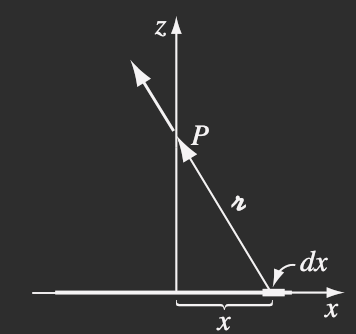
\includegraphics[width=0.3\textwidth]{ex2_2.png}
    \caption{Griffiths Example 2.2}
\end{figure*}
If we treat $\dd q$ as a point particle, then we can use Ex 2.1 likewise but integrate over the line segment. 
\paragraph*{}First we catalog what we know:
\begin{itemize}
    \item Field point $P$ is at $\vb r = z \vu z$
    \item Sources at $\vb r' = x \vu x; \quad \dd \ell' = \dd x$
    \item $\boldscriptr = \vb r - \vb r' = z \vu z - x \vu x$
    \item $\scriptr = \sqrt{x^2 + z^2}$
    \item $\vu \scriptr = \frac{\boldscriptr}{\scriptr} = \frac{z \vu z - x \vu x}{\sqrt{x^2 + z^2}}$
\end{itemize}
The electric field is then (line charge)
\begin{align*}
    \vb E(\vb r) &= \ke \int_{-L}^{+L} \frac{\lambda}{\scriptr^2} \vu\scriptr \dd x = \ke \lambda \int_{-L}^{+L} \frac{z \vu z - x \vu x}{(z^2 + x^2)^{3/2}} \dd x \\
    &= \ke \lambda \qt[z\vu z \int_{-L}^L \frac{\dd x}{(z^2 + x^2)^{3/2}} - \vu x \int_{-L}^L \frac{x \dd x}{(z^2 + x^2)^{3/2}}] \\
    &= \ke \lambda \qt[z\vu z \frac{x}{z^2 \sqrt{z^2 + x^2}}\eval_{-L}^L - \cancel{\vu x \frac{1}{\sqrt{z^2 + x^2}}\eval_{-L}^L}] \\
\end{align*}
we can easily see that the $x$ component is zero through the geometrical symmetry of the line centered at the origin (like Ex 2.1). Simplifying gives us
\[\vb E = \ke \frac{2\lambda L}{z\sqrt{z^2 + L^2}} \vu z\]
Checks and balances:
\begin{itemize}
    \item $\vu z$ is expected!
    \item \[z \gg L \quad \sqrt{z^2 + L^2} \approx z \quad E(P, z\gg L) = \ke \frac{2\lambda L}{z^2}\]
    where we can treat this as a point charge $q = 2\lambda L$ when we are far away.
\end{itemize}

\subsection{Divergence and curl of E: Gauss' Law}

`flux' of field lines
\[ \Phi = \oint_S \vb E \cdot \dd{\vb a} \]
What is $\Phi$ for point charge at origin surrounded by a spherical surface?
\begin{align*}
    \Phi &= \int \vb E \cdot \dd \vb a = \int \ke \frac{q}{r^2} \vu r \cdot \vu r r^2 \sin\theta \dd \theta \dd \phi \\
    &= \frac{q_{enc}}{\epsilon_0}
\end{align*}
\paragraph*{} A bunch of charges surrounded by a surface: \(\vb E_T = \sum \vb E_i\)
\begin{align*}
    \Phi &= \oint \vb E_T \cdot \dd\vb a = \sum_i \oint \vb E_i \cdot \dd \vb a = \sum_i \frac{q_i}{\epsilon_0}
\end{align*}
Thus we have an integral form of Gauss's law:
\begin{align*}
    \boxed{\oint \vb E \cdot \dd\vb a = \frac{Q_{\textrm{enc}}}{\epsilon_0}}
\end{align*}
where $Q = \sum q_i$.
\paragraph*{From the theorem of divergence:}
\[\oint_S \vb v \cdot \dd\vb a = \int_V (\div \vb v) \dd\tau \qand Q = \int_V \rho \dd\tau \]
so
\[\int_V (\div \vb E)\dd\tau = \int_V \rho \dd\tau \to \textrm{good for all volume}\]
therefore we have the differential form of Gauss' Law:
\[\boxed{\div \vb E = \frac{\rho}{\epsilon_0}}\]
\paragraph*{Three ways Gauss's law makes life nice: Gaussian surfaces}
\begin{itemize}
    \item spherical: gaussian sphere
    \item cylindrical: gaussian cylinder
    \item planar: gaussian pillbox
\end{itemize}

\newpage
\lhead{Lecture 4: 9/5/24}

\subsubsection{Applications of Gauss's Law}

\[\int \vb E \cdot \dd\vb a = \frac{q_{enc}}{\epsilon_0} \to \div \vb E = \frac{\rho}{\epsilon_0}\]
\begin{enumerate}
    \item (Simple spherical) What is $\vb E$ outside a uniformly charged solid sphere of radius $R$ and total charge $Q$? The spherical Gaussian surface implies a symmetry where we should \emph{only have a radial component} $\vb E = E_r$.
    \begin{align*}
        \oint \vb E \cdot \dd \vb a &= \frac{Q}{\epsilon_0} \\
        E \oint \dd \vb a = E \cdot 4\pi r^2 &= \frac{Q}{\epsilon_0} \\
        \implies \vb E &= \frac{Q}{4\pi\epsilon_0 r^2} \vu r
    \end{align*}
    where the integral is equivalent to the surface area of the sphere. This is also $\implies$ a field of a \emph{point}.
    \item (Simple cylindrical) A long cylinder (radius $a$) of charge density $\rho = ks$ ($\propto$ distance from axis) where $k$ is a constant and $s$ is the radial distance from the axis. What is $\vb E$ inside the cylinder?
    The cylindrical Gaussian surface has radius $s$ and length $\ell$:
    \begin{align*}
        \oint \vb E _\cdot \dd\vb a = \frac{Q_enc}{\epsilon_0}; \quad Q_{enc} = \int \rho \dd \tau = \int (ks') \dd s' \dd \phi \dd z = \frac{2}{3} \pi k \ell s^3
    \end{align*}
    When using the divergence theorem, note that only the curved part of the cylinder contributes to the flux. Thus,
    \begin{align*}
        \int \vb E \dd \vb a \to E\int \dd a = E (2\pi s \ell) \\
        \implies \vb E = \frac{1}{3\epsilon_0} ks^2 \vu s
    \end{align*}
    If we were to find the field outside the cylinder we would find that the enclosed charge is constant $Q_{enc}$ thus the field is proportional to $1/s$.
    \begin{figure*} [ht]
        \centering
        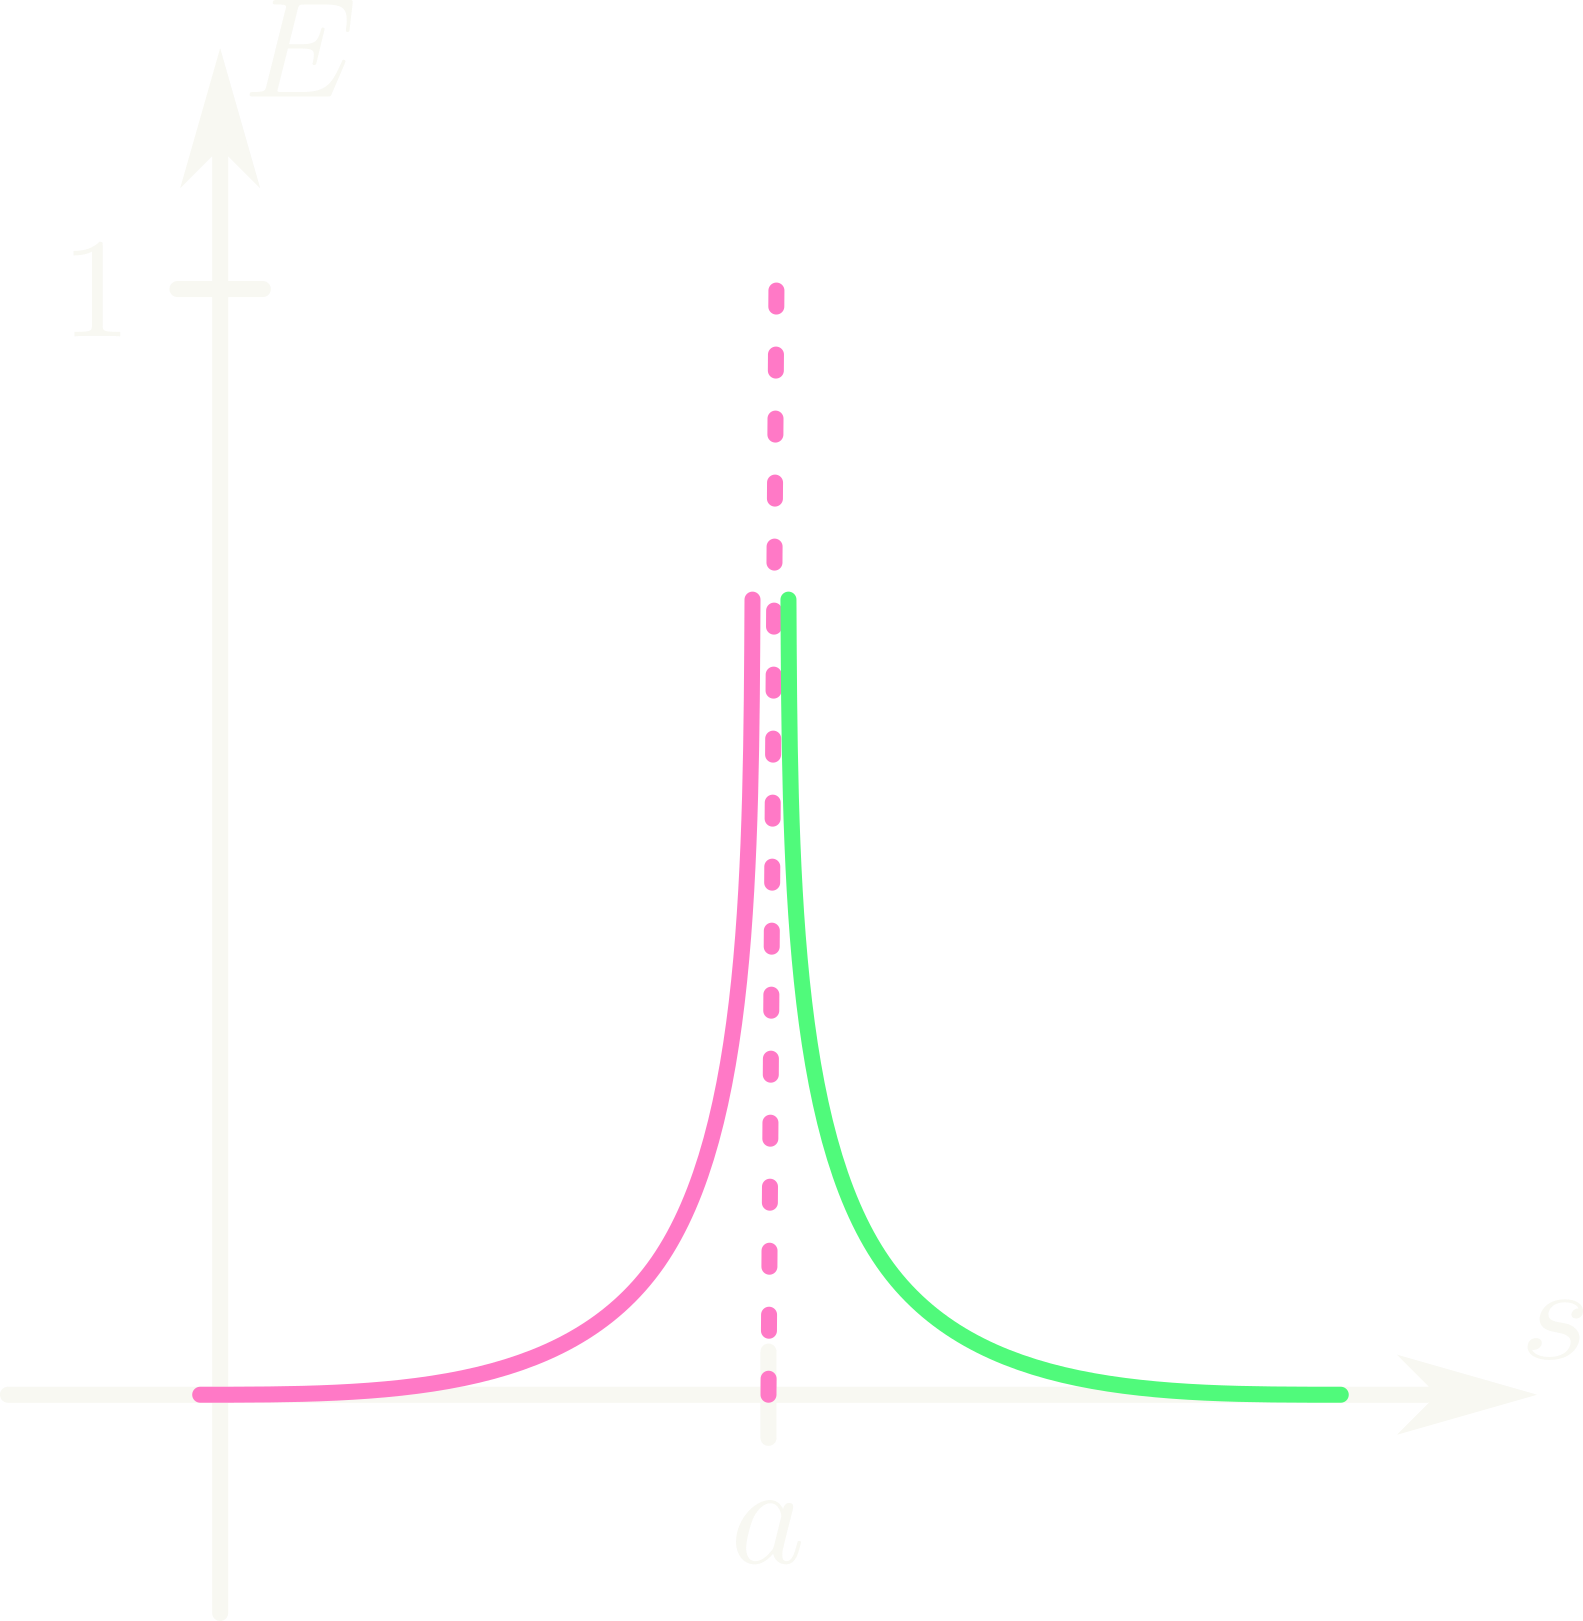
\includegraphics[width=0.3\textwidth]{fig2_3.png}
        \caption{Electric field as a function of $s$}
    \end{figure*}
    \item (Simple infinite plane) with uniform surface charge $\sigma$. Symmetry implies that $\vb E$ is perpendicular to the plane.
    The Gaussian pillbox (either box or cylinder) will have a field of
    \[\vb E = \frac{\sigma}{2\epsilon_0} \vu n \]
\end{enumerate}
\subsubsection{The curl of E}
\[\curl \vb E = 0, \quad \vb E = \frac{1}{4\pi \epsilon_0} \frac{1}{r^2} \vu r \]
calculating
\[\int_a^b \vb E \cdot \dd \ell, \quad \dd \ell = \dd r \vu r + r \dd \theta \vu*\theta + r\sin\theta \dd\phi \vu*\phi\]
So the integral is
\begin{align*}
    \ke \int_a^b \frac{q}{r^2}(\vu r \cdot \vu r) \dd r = \ke \qt(\frac{q}{a} - \frac{q}{b})
\end{align*}
This means:
\begin{itemize}
    \item path independent!
    \item if $a = b$ then $\oint \vb E \cdot \dd \vb\ell = 0$ ($\ell$ is a vector but I don't know how to bold it)
\end{itemize}
We can now use Stokes' theorem: \(\oint \vb v \cdot \dd \ell = \int_S (\curl \vb v) \cdot \dd \vb a\) or
\begin{align*}
    \oint \vb E \cdot \dd\ell = \int_S (\curl \vb E) \cdot \dd \vb a = 0 \implies \curl \vb E = 0
\end{align*}

\subsection{Electric potential}

Any function $f$ with zero curl is the gradient of a scalar function: \(\curl (\grad f) = 0\) (curl of gradient is always 0!)
\[V(\vb r) = - \int_\mathcal{O}^{\vb r} \vb E \cdot \dd \ell\]
implies all paths give some value.

\paragraph*{} $V \sim$ ``electric potential''
\begin{align*}
    V(\vb b) - V(\vb a) &= - \qt(\int_\mathcal{O}^b \vb E \cdot \dd \ell) - \qt(-\int_\mathcal{O}^a \vb E \cdot \dd\ell) \\
    &= - \int_\mathcal{O}^b - \int_\mathcal{a}{O} \vb E \cdot \dd\ell \\
    &= - \int_a^b \vb E \cdot \dd \ell
\end{align*}
And from the fundamental theorem for gradients: \(T(\vb b) - T(\vb a) = \int_a^b (\grad T) \cdot \dd\ell \)
\[\implies \vb E = -\grad V \]
\begin{enumerate}
    \item [i] ``potential'' is a terrible name
    \item [ii] $\vb E = (E_x, E_y, E_z)$ vs $V$ with only \emph{one} value at every point in space! Otherwise we would have to deal with
    \[(\curl \vb E)_x = \pdv{E_z}{y} - \pdv{E_y}{z} = 0\]
    \item [iii] \[V'(\vb r) = -\int_{O'}^{\vb r} \vb E \cdot \dd\ell = - \int_{O'}^O \vb E \cdot \dd\ell - \int_O^{\vb r} \vb E \cdot \dd\ell = C + V(\vb r) \]
    $\implies \vb E = - \grad V$
\end{enumerate}

\newpage
\lhead{Lecture 5: 9/10/24}
\paragraph*{Electric Potential cont.}

\subsubsection{Poisson's and Laplace's equations} The divergence and curl of $\vb E$ in terms of the potential $V$:

\begin{itemize}
    \item Divergence: \(\div \vb E = \div (-\grad V) = -\laplacian V\), or \textbf{Poisson's equation}:
    \begin{align*}
        \boxed{\laplacian V = -\frac{\rho}{\epsilon_0}}
    \end{align*}
    and in regions of no charge $\rho = 0$ we have \textbf{Laplace's equation}:
    \[\boxed{\laplacian V = 0}\]
    \item Curl: It's always zero, which doesn't give us any info about $V$\dots
\end{itemize}

\subsubsection{Potential of localized charge distributions}

For a point charge $q$ we can easily find the potential using the electric field $\vb E = \frac{q}{4\pi\epsilon_0 r^2} \vu r$:
\begin{align*}
    V(r) &= -\int_O^r \vb E \cdot \dd \vb*\ell = - \ke \int_\infty^r \frac{q}{r'^2} \dd r'\\
    &= \ke \frac{q}{r}
\end{align*}
where in general, the potential of a point charge is
\begin{align*}
    V(\vb r) = \ke \frac{q}{\scriptr}
\end{align*}
And using the principle of superposition, the potential of a collection of charges can be a sum
\begin{align*}
    V(\vb r) = \ke \sum_i \frac{q_i}{\scriptr_i}
\end{align*}
or for a continuous charge distribution, and integral:
\begin{align*}
    V(\vb r) = \ke \int \frac{1}{\scriptr} \dd q
\end{align*}
e.g. for a volume charge distribution:
\begin{align*}
    \boxed{
        V(\vb r) = \ke \int \frac{\rho(\vb r')}{\scriptr} \dd \tau'
    }
\end{align*}

\subsubsection{Boundary conditions}

From the Gaussian pillbox the E-field is given by Gauss's law:
\[\oint_S \vb E \cdot \dd \vb A = \frac{Q_{\textrm{enc}}}{\epsilon_0} = \frac{\sigma A}{\epsilon_0}\] 
and the only components that contribute to the field are the top and bottom:
\begin{align*}
    \vb E_{\textrm{above}}^{\perp} - \vb E_{\textrm{below}}^\perp = \frac{\sigma}{\epsilon_0} \vu n
\end{align*}
But we can also use the path integral of the E-field (which should be zero):
\begin{align*}
    \oint \vb E \cdot \dd \vb*\ell = 0
\end{align*}
so the parallel components should be equal:
\begin{align*}
    \vb E_{\textrm{above}}^{\parallel} - \vb E_{\textrm{below}}^\parallel = 0 \\
    \implies \boxed{E_{\textrm{above}}^{\parallel} = E_{\textrm{below}}^\parallel}
\end{align*}
This also implies that the potential ``$V$ is continous across boundaries'':
\begin{align*}
    V_{\textrm{above}} = V_{\textrm{below}}
\end{align*}
which also implies the gradient of the potential is
\begin{align*}
    \grad V_{\textrm{above}} - \grad V_{\textrm{below}} = -\frac{\sigma}{\epsilon_0} \vu n
\end{align*}

\subsection{Work and energy in electrostatics}

$[V] = \si{J/C}$ = energy/charge, so the work is equivalent to
\begin{align*}
    W = Q V(\vb r)
\end{align*}

\subsubsection{Energy of point charge distribution}
\paragraph*{Collection of 3 charges} First we assume we start with $W_1 = 0$,
or we are bringing the two other charges towards $q_1$; Work done to bring in $q_2 = V_1 q_2 = W_2$;
\begin{align*}
    W_3 &= V_1 q_3 + V_2 q_3 \\
    &= \ke \frac{q_1 q_3}{r_{13}} + \ke \frac{q_2 q_3}{r_{23}} \\
    &= \ke q_3 \qt(\frac{q_1}{r_{13}} + \frac{q_2}{r_{23}})
\end{align*}
where we can use the superposition principle to find the total work:
\begin{align*}
    W = W_1 + W_2 + W_3
\end{align*}

\paragraph*{In general}
\begin{align*}
    W &= \ke \sum_{i=1}^n \sum_{j>i}^n \frac{q_i q_j}{r_{ij}} \\
    &= \frac{1}{2} \ke \sum_{i=1} \sum_{j\neq i} \frac{q_i q_j}{r_{ij}} \\
    &= \frac{1}{2} \ke \sum_{i=1} q_i \sum_{j\neq i} \frac{q_j}{r_{ij}} \\
    &= \frac{1}{2} \sum_{i=1} q_i \qt[\sum_{j\neq i} \ke \frac{q_j}{r_{ij}}]
\end{align*}
where the term in the brackets is the potential energy due to all other charges, $[\;] = V(\vb r_i)$, thus
\begin{align*}
    W = \frac{1}{2} \sum_{i=1} q_i V(\vb r_i)
\end{align*}

\subsubsection{Energy of continuous charge distribution}
\begin{align*}
    W = \frac{1}{2} \int \rho V \dd \tau
\end{align*}
but what if we don't know the potential? First using Gauss's law:
\begin{align*}
    \rho = \epsilon_0 \div \vb E
\end{align*}
so the work done is (using integration by parts):
\begin{align*}
    W &= \frac{\epsilon_0}{2} \int (\div \vb E) V \dd\tau \\
    &= \frac{\epsilon_0}{2} [-\int \vb E(\grad V) \dd\tau + \oint V\vb E \cdot \dd \vb A] \\
    &= \frac{\epsilon_0}{2} [\int E^2 \dd \tau + \oint V \vb E \cdot \dd \vb A]
\end{align*}
but we know that
\begin{itemize}
    \item $E \propto \frac{1}{r^2} \quad \dd\tau \propto r^3$
    \item $V \propto \frac{1}{r} \quad \dd A \propto r^2$
\end{itemize}
So the second surface integral term goes to 0 much faster, thus
\begin{align*}
    W = \frac{\epsilon_0}{2} \int E^2 \dd \tau
\end{align*}

\newpage
\lhead{Lecture 6: 9/12/24}

\paragraph*{Energy Review:}
\begin{align*}
    W = \frac{1}{2} \sum q_i V(\vb r_i) \\
    W = \frac{\epsilon_0}{2} \int E^2 \dd \tau
\end{align*}
Where did we go wrong in going from the point charge distribution to the continuous distribution?

\subsubsection{Comments on Electrostatic energy}

Energy of a point charge?:
\begin{align*}
    W = \frac{\epsilon_0}{2} \int \frac{q^2}{(r^2)^2} r^2 \sin\theta \dd r \dd\theta \dd\phi = \infty
\end{align*}
Uh oh, as $r \to 0$ the energy goes to infinity! And this problem persists everywhere. (Solution is renormalization\dots)

\paragraph*{Where is the energy stored?}
\begin{itemize}
    \item In the first case: we have a charge in a potential (from other charges); somehow the relative position of the charge implies its ``electric potential''
\end{itemize}
We don't really know where it is, but we can book keep this energy i.e. $\rho, V, E$

\paragraph*{Superposition (again)} If we try to superimpose two electric fields,
\begin{align*}
    W = \frac{\epsilon_0}{2} \int \abs{\vb E_1 + \vb E_2}^2 \dd \tau
\end{align*}
the terms in the integral are 
\begin{align*}
    E_1^2 + E_2^2 + 2\vb E_1 \cdot \vb E_2
\end{align*}
so
\begin{align*}
    W \neq W_1 + W_2
\end{align*}

\subsection{Conductors in electrostatics}

\subsubsection{Basic Properties}

What is a conductor? Material where charge can move; in the perfect case, the charges move freely and the resistance goes to zero $R \to 0$.
Thus no \textit{resistance} to the motion of charge.

\begin{enumerate}
    \item [i] $\vb E = 0$ inside a conductor
    
    if $E + q \to \vb F = q \vb E$: a charge in a field $\to$ charges move to canncel $\vb E_{\textrm{in}}$
    \item [ii] $\rho = 0$ inside a conductor; so from divergence
    \begin{align*}
        \div \vb E = \frac{\rho}{\epsilon}, \qif \vb E = 0,\; \rho = 0
    \end{align*}
    \item [iii] any non-zero $\rho$ resides on surface (only in 3D);
    in 2D \& 1D, its not exactly at the boundary, but quickly peaks and decays before the boundary.
    \item [iv] conductors are equipotentials
    \item [v] $\vb E$ is perpendicular to a surface outside the conductor
\end{enumerate}

\paragraph*{The silly experiment:} An aluminum beverage can (of ingenious design) is a conductor, i.e., it has free electrons.
The plastic rod is given negative charge (via cloth/wool) and when it is brought near the can, the can moves towards the rod.

How does the can move, even though it has no charge? The rod induces a charge by pushing the negative charges away from the can.
Then the positive charges close to the rod are attracted hence the attractive movement (force).

\subsubsection{Induced charge distributions}

\begin{figure}[ht]
    \centering
    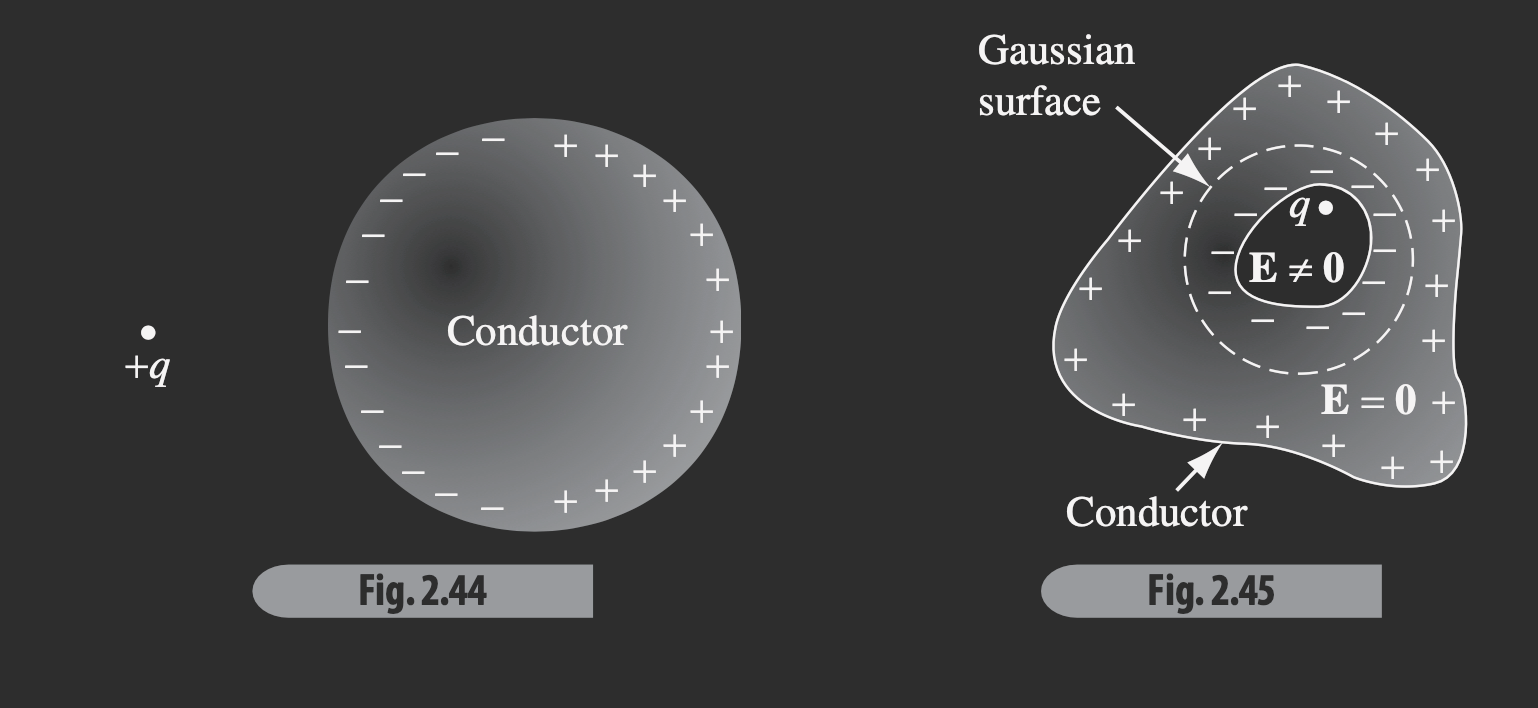
\includegraphics[width=0.5\textwidth]{fig2_44.png}
    \caption{From Griffiths}
\end{figure}
\paragraph*{Case 1:} A point charge in a cavity surrounded by a conductor
\begin{itemize}
    \item Flux $\Phi = \int \vb E \dd\vb A \neq 0$ for a Gaussian surface in the cavity
    \item $\Phi = \int \vb E \dd\vb A = 0$ for a surface where that encloses no charge (positive point charge cancels negative charges surrounding it in the conductor)
    \item $\int \vb E \dd\vb A = \frac{q_{\textrm{enc}}}{\epsilon_0} = \frac{q}{\epsilon_0}$ for a Gaussian surface outside the conductor
\end{itemize}

\paragraph*{Case 2:} Spherical conductor, with a weird cavity containing a point charge $+q$

What is $\vb E (\vb P)$ at $\vb P$ for $P > r$ (outside the conductor)? The electric field will uniformly distribute itself in the conductor, so
\begin{align*}
    \vb E = \ke \frac{q}{r^2} \vu r
\end{align*}
What about a point charge $+q$ outside the conductor, what is the E-field in the cavity? It may put minus charges close, and plus charges away from further away on the surface of the conductor\dots
but in the cavity, you can't transmit information in the cavity since the E-field is zero inside a conductor.
Screening out an electric field AKA the Faraday cage.

\subsubsection{Capacitors}

Imagine 2 conductors (of weird shapes) with charges $+Q$ and $-Q$ has a potential of $+V$ and $-V$ respectively.
The potential difference (Theorem of gradients) is
\begin{align*}
    \Delta V = V_+ - V_- = -\int_{(-)}^{(+)} \vb E \cdot \dd\vb*\ell
\end{align*}
where we know that there is an electric field $\vb E \propto Q$ or more precisely from Coloumb's law:
\begin{align*}
    \vb E = \ke \int \frac{\rho}{\scriptr^2} \vu\scriptr \dd \tau
\end{align*}
thus
\begin{align*}
    \Delta V \propto Q \implies C \equiv \frac{Q}{\Delta V}
\end{align*}
where $C$ is the ``capacitance''.

\paragraph*{Example: Parallel plate capacitor} Two very large plates with area $A$, charge $+Q$ \& $-Q$, a separation $d$ such that $d \ll \sqrt{A}$,
and the surface charge density is $\sigma_{\pm} = \pm \frac{Q}{A}$

We can easily find the electric field of a plate $\vb E = \frac{\sigma}{2\epsilon_0} \vu n$,
and in the presence of two oppositely charged plates, there is only an electric field between the plates with double the magnitude:
\begin{align*}
    E = \frac{\sigma}{\epsilon_0}
\end{align*}
The potential difference is then
\begin{align*}
    \Delta V &= \int \vb E \cdot \dd\vb*\ell \\
    &= \frac{\sigma}{\epsilon_0} d = \frac{d}{\epsilon_0} \frac{Q}{A}
\end{align*}
so the capacitance of the parallel plates is
\begin{align*}
    C_\parallel = \frac{Q}{\Delta V} = \frac{\epsilon_0 A}{d}=[]
\end{align*}
\end{document}